\documentclass[conference]{IEEEtran}
\IEEEoverridecommandlockouts
% The preceding line is only needed to identify funding in the first footnote. If that is unneeded, please comment it out.
%Template version as of 6/27/2024

\usepackage{cite}
\usepackage{amsmath,amssymb,amsfonts}
\usepackage{algorithmic}
\usepackage[dvipdfmx]{graphicx}
\usepackage{textcomp}
\usepackage{xcolor}
\def\BibTeX{{\rm B\kern-.05em{\sc i\kern-.025em b}\kern-.08em
    T\kern-.1667em\lower.7ex\hbox{E}\kern-.125emX}}
\begin{document}

\title{量子最適化}

\author{\IEEEauthorblockN{1\textsuperscript{st} Given Name Surname}
\IEEEauthorblockA{\textit{dept. name of organization (of Aff.)} \\
\textit{name of organization (of Aff.)}\\
City, Country \\
email address or ORCID}
\and
\IEEEauthorblockN{2\textsuperscript{nd} Given Name Surname}
\IEEEauthorblockA{\textit{dept. name of organization (of Aff.)} \\
\textit{name of organization (of Aff.)}\\
City, Country \\
email address or ORCID}
\and
\IEEEauthorblockN{3\textsuperscript{rd} Given Name Surname}
\IEEEauthorblockA{\textit{dept. name of organization (of Aff.)} \\
\textit{name of organization (of Aff.)}\\
City, Country \\
email address or ORCID}
}

\maketitle

\begin{abstract}
This document is a model and instructions for \LaTeX.
This and the IEEEtran.cls file define the components of your paper [title, text, heads, etc.]. *CRITICAL: Do Not Use Symbols, Special Characters, Footnotes, 
or Math in Paper Title or Abstract.
\end{abstract}

\begin{IEEEkeywords}
component, formatting, style, styling, insert.
\end{IEEEkeywords}

\section{イントロダクション}
\subsection{背景と目的}
組合せ最適化問題とは,複数の制約があり,これらを満たす時に与えられた集合の中から目的関数を最大化または最小化する最適な解を見つける問題である.代表的な例として巡回セールスマン問題,ナップサック問題,スケジューリング問題等がある.しかし,最適解を見つけることは困難である.なぜなら,問題のサイズにより解の数が膨大になり現実的な時間内で求めることが難しいからである.したがって,組合せ最適化問題の新しい解法として注目を集めている量子化技術が使われることが多い.

量子アニーリングは,最適化問題を数式で表現するQUBO(Quadratic Unconstrained Binary Optimization)モデルとIsingモデルと呼ばれるエネルギー関数があり,そのエネルギーを最小化にすることを目的として最適化を図る.さらに,量子アニーリングは実用化が進んでおり,D-Wave社が商業用のアニーリングマシンを開発している.この技術により,従来の手法では解決が困難である組合せ最適化問題が改めて注目を集めている.

本論文で扱うスケジューリング問題は,ジョブショップスケジューリング問題を対象とし,各タスクを処理するのにかかるリソースコストと前のタスクが処理し終えた後,次のタスクを処理し始めるための待ち時間を最小化を目的としている.また,ジョブを増やした際に,どの程度までジョブを増やせるか,その際のハイパーパラメータが見つかるのかついても検証を行う.

\section{基礎概念}
\subsection{フローショップスケジューリング問題}
フローショップスケジューリング問題は,複数の工程から構成される複数のジョブを処理するためのスケジューリング問題である.ジョブは複数の工程によって構成され,工程毎に指定された共有リソースを利用する必要がある.各ジョブにおける一つの処理工程をタスクと呼ぶ.\cite{b1}

本論文で扱っているスケジューリング問題を以下にまとめる.

\begin{itemize}
\item ジョブの数は15個、1つのジョブには3つのタスクがある.
\item 各ジョブは複数のタスクを順番に経る必要があり,各タスクは特定のマシンリソースを利用する.
\item 各タスクには処理を終えるまでの上限時間と最低でも指定された時間内に処理を始める下限時間があり,前のタスクの上限時間と次のタスクが下限時間の差が定められた制限時間内に収まるようにリソースを利用する.
\end{itemize}

%\begin{figure}[htbp]
%\centerline{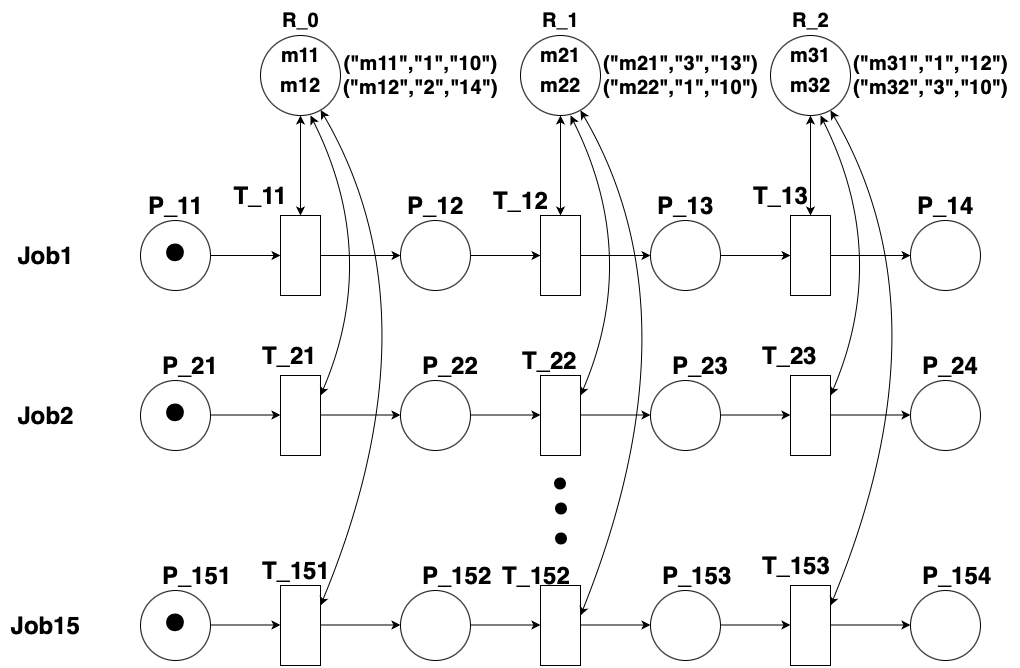
\includegraphics{fsp.png}}
%\caption{Example of a figure caption.}
%\label{fig}
%\end{figure}

\subsection{QUBOモデル}
QUBOモデルは最適化問題を表現するモデルの一種である.変数が0か1の値を取るバイナリ変数$q_i$として表現される.また,バイナリ変数の係数が実数値として$Q_{i,j}$と表現される.QUBOモデルの式を以下に示す.

\begin{align}
H = \sum_{i,j} Q_{i,j} q_i q_j
\end{align}

\section{評価実験}
\subsection{実験環境}
ハードウェア構成
\begin{itemize}
\item CPU:Apple M1 3.2 GHz
\item メモリ:8 GB
\item ストレージ:256 GB SSD
\end{itemize}  

\vspace{\baselineskip}

ソフトウェア構成 
\begin{itemize}
\item OS:macOS Sonoma 14.3.1
\item プログラミング言語とライブラリ:Python 3.10.14,openjij 0.9.2,re 2.2.1,pyqubo 1.4.0
\item ストレージ:256 GB SSD
\end{itemize}

\subsection{実験方法}

\subsection{結果}

\section{考察}

\section{結論}

\begin{thebibliography}{00}
\bibitem{b1} 新城 巧也, ``ペトリネットに基づく実用性を考慮した組合せ最適化問題に対する量子インスパイアード最適化,'' 2022年3月
\end{thebibliography}

\end{document}
